\documentclass[12pt,a4paper,oneside]{report}
\usepackage[T1]{fontenc}
\usepackage[utf8]{inputenc}
\usepackage[margin=3cm]{geometry}
\usepackage{graphicx}
\usepackage{booktabs}
\usepackage[hyphens]{url}
\usepackage{hyperref}
\usepackage{natbib}
\usepackage{fancyhdr}
\usepackage{microtype}
\pagestyle{fancy}
\usepackage[normalem]{ulem}
\usepackage{textcomp}
\usepackage{amsmath}
\usepackage{amssymb}
\setlength{\parindent}{0pt}
\setlength{\parskip}{6pt}

\setlength{\emergencystretch}{5em}
\sloppy
\title{Untitled}
\author{}
\date{\today}

\begin{document}

\begin{figure}[htbp]
  \centering
  
\includegraphics[width=3.70cm]{media/image1.jpeg}
  \caption{drawingObject1}
\end{figure}

\textbf{KYAMBOGO                                                                                                                                                           UNIVERSITY FACULTY OF ENGINEERING}


\textbf{DEPARTMENT OF ELECTRICAL AND ELECTRONICS ENGINEERING}


\textbf{BACHELOR OF ENGINEERING IN TELECOMMUNICATIONS ENGINEERING RESEARCH PROPOSAL}








\textbf{THE AUTOMATED ROUTER MANAGEMENT SYSTEM TO IMPROVE THE LIMITATIONS OF CGNAT}




\textbf{By}


\textbf{MUHWEZI MARK}


\textbf{REGISTRATION NUMBER: 22/U/ETD/0996/GV}


\textbf{Supervisor: Dr. MUGERWA DICKSON}




\textit{\textbf{A report submitted to the Electrical and Electronics Engineering Department, Kyambogo University, in fulfillment of the requirements for the degree of Bachelor of Engineering in Telecommunications Engineering}}


\clearpage







\textbf{Declaration of Authorship}




I Muhwezi Mark hereby declare that this final year project report is an original and authentic work that has been carried out by me under the supervision of Dr. Mugerwa Dickson as part of my course requirements for the Bachelor of Engineering in Telecommunications Engineering of Kyambogo University




I confirm that this report has not been submitted previously for any other academic award or qualification. All sources of information used in this report have been duly acknowledged through appropriate citations and references




I also confirm that the work presented in this report is free from any plagiarism and any contribution made by others to this work has been duly acknowledged.


I acknowledge that the copyright of this report belongs to the academic institution and that no part of this report may be reproduced or transmitted in any form or by any means, electronic, mechanical, photocopying, recording or otherwise, without the prior written permission of the academic institution.








Date: Monday 29th June 2026


\clearpage



\textbf{Approval}


This final year project has been done under the supervision and has been submitted to the Faculty of Engineering of Kyambogo University for examination with approval


Supervisor: Dr. Mugerwa Dickson




Sign:




Date:


\clearpage



\textbf{Dedication}


I dedicate this work to my beloved families and friends, whose unwavering support, encouragement and sacrifices have been the foundation of our academic journey. To my family, for instilling in me the value of education and perseverance and to our friends and colleagues for their motivation and inspiration throughout the course of the project. This work is also dedicated to all students and researchers striving to use technology to create innovative solutions for real world challenges.


\clearpage

\textbf{Acronyms}


This is a list of acronyms used whilst this report


NAT  - Network Address Translation


CGNAT - Carrier Grade Network Address Translation


RFC  - Requests for Comments


IPv4  - Internet Protocol Version 4


IPv6  - Internet Protocol Version 6


QoS  - Quality of Service


AWS  - Amazon Web Services


RSA  - Rivest Shamir Adleman


SSH  -Secure Shell


VoIP  - Voice Over Internet Protocol


NAC   - Network Access Control


USSD  - Unstructured Supplementary Service Data


MSISDN - Mobile Station International Subscriber Directory Number


SMS  - Short Message Service


Email  - Electronic Mail


SS7  - Signaling System No. 7


JWT  - JSON Web Token


JSON  - JavaScript Object Notation


TCP  - Transmission Control Protocol


HTTP  - Hypertext Transfer Protocol


ISP  - Internet Service Provider


WLAN  - Wireless Local Area Network


AAA  - Authentication, Authorization and Accounting


REST   - Representational State Transfer


AES  - Advanced Encryption System


CPE  - Customer Premises Equipment


API  - Application Programming Interface


3GPP  - 3rd Generation Partnership Project


HMAC - Hash-based Message Authentication Code


ER  - Entity Relationship


URL  - Uniform Resource Locator


SSL  - Secure Sockets Layer


CORS  - Cross Origin Resource Sharing


UI  - User Interface


\textbf{URL Links}


These are links that are associated to the project prototype


\begin{itemize}
  \item Database Er Diagram - \href{https://terraconnect-er-diagram.web.app}{https://terraconnect-er-diagram.web.app}
  \item TerraConnect Uganda Dashboard UI - \href{https://terraconnect-uganda.web.app}{https://terraconnect-uganda.web.app}
  \item Backend URL -- \href{https://quicknetwifi.org/terraconnect}{https://quicknetwifi.org/terraconnect}
\end{itemize}



\clearpage

\uline{\textbf{Nomenclature}}


The name \textbf{TerraConnect Uganda} was deliberately chosen to reflect the core purpose, geographical context, and technical vision of this project.


\textbf{"Terra"} is derived from the Latin word for \textit{earth} or \textit{land}, symbolising the physical network infrastructure routers, cables, and devices that form the foundation of internet connectivity across communities. It represents the grounded, real-world nature of the problem being addressed: the challenge of managing distributed physical network equipment remotely and reliably.


\textbf{"Connect"} signifies the system's primary function establishing and maintaining secure, stable, and seamless connections between geographically dispersed MikroTik routers and a centralised management platform. It further alludes to the WireGuard VPN tunnels that form the backbone of the system's communication architecture, bridging devices across diverse and often constrained network environments such as those imposed by Carrier-Grade NAT (CGNAT).


\textbf{"Uganda"} anchors the project in its operational context, acknowledging that the system was designed, developed, and tested with the specific networking landscape of Uganda in mind including the prevalence of ISPs operating under CGNAT conditions, limited static IP availability, and the growing demand for scalable remote network management solutions in the region.


Together, \textbf{TerraConnect Uganda} embodies a system that connects the physical network infrastructure of Uganda through a secure, intelligent, and remotely accessible platform bridging the gap between network administrators and the routers they manage, regardless of geographical distance or network constraints.


\clearpage





\uline{\textbf{List of Figures}}










\clearpage



\uline{\textbf{List of Tables}}












 




\tableofcontents
\clearpage

\textbf{Abstract}


The widespread adoption of Carrier-Grade NAT (CGNAT) by Internet Service Providers, driven by global IPv4 address exhaustion, has created a significant challenge for the remote management of customer premises equipment, such as MikroTik routers (Cloudflare, 2022). While CGNAT effectively conserves public IP addresses, it prevents unsolicited inbound connections, thereby breaking traditional methods for direct configuration, monitoring, and troubleshooting (Al-Ani \& Othman, 2020). Existing workarounds, including static IP leasing, port forwarding, or reliance on vendor-specific relay services like MikroTik's Back-to-Home (BTH), are often costly, insecure, or lack the flexibility required for scalable, automated deployments (MikroTik, 2023; Sokolov \& Komarov, 2022).




This project presents a novel system that integrates a Rust-based backend with the RouterOS API and WireGuard tunnels to provide a secure, cost-effective, and reliable solution for remote access to MikroTik routers behind CGNAT. The system automates the provisioning of WireGuard peers on both the routers and a public cloud endpoint (hosted on AWS EC2), securely managing cryptographic keys and the entire tunnel lifecycle (Donenfeld, 2020). A lightweight web interface, developed with modern frontend technologies, provides administrators with real-time visibility into router status, peer activity, and tunnel health.




The solution was evaluated in real-world scenarios, including routers behind CGNAT, on public IP networks, and on dynamic LTE connections. The results demonstrate that by leveraging persistent outbound WireGuard connections, routers remain consistently accessible and manageable despite CGNAT restrictions. A comparative analysis with MikroTik's BTH service highlights the system's advantages in terms of operational flexibility, independence from vendor infrastructure, and its inherent potential for scalable, multi-tenant deployments.


The findings confirm that the synergistic combination of Rust chosen for its performance and


memory safety (Davidson et al., 2021) the RouterOS API, and WireGuard provides a high-performance and practical approach to overcoming CGNAT limitations. This project offers a valuable, open-source contribution to network operators, enterprises, and researchers in the fields of network automation and secure remote access.


\clearpage



\textbf{Acknowledgements}


All glory and gratitude are first rendered to the Almighty God, whose grace, wisdom, and strength sustained us throughout the course of this project from its inception to its successful completion.


We wish to express our profound gratitude to our supervisor, Dr. Mugerwa Dickson, for his unwavering guidance, rigorous intellectual engagement, and consistent support during both the research and simulation phases of this work. His depth of expertise and constructive critique were instrumental in shaping this project to its present standard.


Our sincere appreciation is further extended to the academic and administrative staff of the Department of Electrical and Electronics Engineering, Kyambogo University, for fostering a stimulating and supportive learning environment throughout our academic programme.


We also acknowledge our colleagues and peers whose contributions through scholarly discussions, suggestions, and moral encouragement enriched this work in no small measure.


Finally, we are deeply indebted to our families for their unconditional love, patient understanding, and steadfast encouragement a constant source of strength and motivation throughout this journey.


MUHWEZI MARKJune 2026






\chapter{CHAPTER 1: INTRODUCTION}

\section{1.1 Background of the study}

In recent years, the global exhaustion of IPv4 addresses has led many Internet Service Providers (ISPs) to adopt Carrier-Grade Network Address Translation \textbf{(CGNAT) }as a way of extending the usability of the limited IPv4 space. While CGNAT helps ISPs conserve public IP addresses, it introduces a major limitation where devices behind CGNAT cannot be directly accessed from the internet (Al-Ani \& Othman, 2020). This creates significant challenges for remote network management, device monitoring, and configuration, especially for organizations that rely on remote access to their routers and network equipment (Herzberg et al., 2022).


MikroTik routers, powered by RouterOS, are widely used in both small and large-scale networks due to their flexibility, affordability, and powerful features. Network administrators typically manage MikroTik routers through public IP access\textbf{, }VPNs, or third-party cloud services such as MikroTik's \textit{Cloud Hosted Router (CHR) }or \textit{Back-To-Home (BTH) (Mikrotik, 2023)}. These solutions often have limitations and they may require static public IPs, rely on vendor-controlled infrastructure, or introduce privacy and scalability concerns (Sokolov \& Komarov, 2022).


At the same time, the increasing need for secure, efficient, and automated remote management has led to the exploration of modern programming languages and VPN technologies. Rust, a systems programming language known for its safety, speed, and concurrency, has become a preferred choice for developing high-performance backend systems (Davidson et al., 2021; Mozilla Foundation, 2023). On the other hand, WireGuard, a lightweight and cryptographically secure VPN protocol, has emerged as a modern alternative to traditional VPNs like IPSec and OpenVPN due to its simplicity and superior performance (Donenfeld, 2020; Kumar \& Singh, 2021; Wright \& Samuels, 2021).


With this Integration of Rust\textbf{, }WireGuard\textbf{, }and RouterOS API we create an opportunity to develop a system that allows remote router access even under CGNAT, without relying on public IPs or centralized cloud services (MikroTik, 2024). This system can enable routers to initiate secure outbound connections to a central Rust-based backend server through WireGuard tunnels, effectively bypassing CGNAT restrictions while maintaining encryption, authentication, and data integrity (Fielding, 2000; Gong et al., 2018).




\section{1.2 Problem Statement}

In Uganda and many other regions grappling with IPv4 address exhaustion, Internet Service Providers (ISPs) have widely adopted Carrier-Grade Network Address Translation (CGNAT) as a necessary measure to conserve the dwindling supply of public addresses (Cloudflare, 2022). While CGNAT is effective for extending the lifespan of IPv4, it introduces a critical operational barrier: it renders devices on the customer premises, such as routers, inaccessible to direct inbound connections from the public internet. This fundamentally breaks traditional methods of remote management, real-time monitoring, and the establishment of secure site-to-site VPNs (Al-Ani \& Othman, 2020; Herzberg et al., 2022).


MikroTik routers, which are ubiquitous in these markets due to their affordability and flexibility, support management through Winbox, WebFig, and a proprietary API. However, all these interfaces inherently depend on direct IP reachability, which is obstructed by CGNAT (MikroTik, 2024). Existing workarounds, such as purchasing static public IPs, configuring complex port forwarding rules, or using dynamic DNS services, are either financially prohibitive, inherently insecure, or too impractical to deploy and maintain at scale (Sokolov \& Komarov, 2022).


Consequently, a significant gap exists in the current landscape. While vendor-specific


solutions like MikroTik's Back-To-Home (BTH) VPN offer convenience, they create vendor lock-in, lack programmability for automation, and are not supported on the vast installed base of older RouterOS hardware (MikroTik, 2023). Therefore, there is a pressing need for a unified, open, and programmable system that empowers network operators with a low-cost, scalable, and vendor-independent solution.




This project aims to address this critical gap by designing and implementing an automated management system. The system will leverage a Rust-based backend server, hosted on a cloud virtual private server (e.g., Amazon EC2) with a stable public IP, to act as a central rendezvous point. The core of the solution will automate the provisioning and lifecycle of secure WireGuard tunnels (Donenfeld, 2020), enabling MikroTik routers behind CGNAT to initiate outbound connections. This architecture will ensure persistent reachability, enabling centralized configuration, monitoring, and management without the need for public IPs on the client routers, thereby solving a fundamental operational challenge introduced by CGNAT.




6


\section{1.3 Objectives}

\textbf{The main objective of the study}


The main objective of this project is to design, implement, and evaluate a secure and efficient system for remote management of MikroTik routers located behind CGNAT, by integrating a Rust-based backend, WireGuard VPN tunnels, and RouterOS API automation\textbf{.}




\textbf{Specific objectives}




I. To analyze the technical constraints imposed by CGNAT


II. To design and develop a secure backend service in Rust III. To establish and automate secure WireGuard tunnels




\section{1.4 Justification of The System}

The growing adoption of Carrier-Grade Network Address Translation \textbf{(CGNAT) }by Internet Service Providers (ISPs) has made remote management of customer premises routers increasingly difficult. Traditionally, administrators could directly access routers using public IP addresses for configuration, monitoring, and troubleshooting. However, CGNAT limits inbound connections, isolating routers behind shared Ips and creating significant NAT traversal challenges (Herzberg et al., 2022). This presents a major challenge for network administrators, ISPs, and enterprise IT departments that rely on remote management and monitoring (Al-Ani \& Othman, 2020).


Existing solutions, such as MikroTik's Back-To-Home (BTH) and Cloud Hosted Router \textbf{(}CHR\textbf{)}, provide partial workarounds but come with limitations including high setup complexity, dependency on MikroTik's cloud infrastructure, or lack of full automation and customization capabilities (Mikrotik, 2023; Sokolov \& Komarov, 2022). These issues highlight the need for a flexible, self-hosted, and secure alternative that can be tailored for specific network environments.


This project is justified on both technical and practical grounds. From a technical perspective, the integration of Rust, RouterOS API, and WireGuard VPN offers an innovative and high-performance solution for overcoming CGNAT-related access restrictions. Rust's memory safety, concurrency, and speed make it ideal for building secure backend systems that can handle multiple routers efficiently (Davidson et al., 2021; Mozilla Foundation, 2023). WireGuard's lightweight encryption and ease of deployment enable seamless creation of VPN tunnels through NATs, ensuring persistent and secure communication between routers and the central management server (Donenfeld, 202; Wright \& Samuels, 2021). Furthermore, the programmability of Mikrotik devices via the RouterOS API is a key enabler for this automation (Wijaya et al., 2020).


From a practical standpoint, the project addresses a real-world problem faced by network engineers in Uganda and globally, where CGNAT is increasingly common due to IPv4 exhaustion (Cloudflare, 2022). The system reduces operational costs by eliminating reliance on third-party cloud routing services and provides ISPs and organizations with full control over their infrastructure, aligning with principles of self hosted and autonomous system design (Fielding, 2000). Furthermore, it contributes to local capacity building in secure network automation and Rust-based backend development, areas that are both modern and in high demand.




This project all in all is justified as a cost-effective, secure, and technically advanced approach to remote router management that empowers administrators to operate beyond CGNAT constraints. It aligns with the current trends in network automation\textbf{, }cybersecurity, and self-hosted infrastructure management (Ashraf \& Latif, 2020; Schmidt \& Wuttke, 2019), making it a relevant and valuable contribution to both academic research and practical telecommunications applications.


\section{1.5 Significance of The System}

This project is significant for its direct contribution to solving a critical operational problem in modern networking. The significance of this study is as follows:




\textbf{Enables Secure Remote Management Behind CGNAT}


The system provides a reliable method for continuous, secure remote access to MikroTik routers operating behind CGNAT. This allows administrators to perform configuration, monitoring, and troubleshooting from any location, without the need for a public IP address on the client router. This capability is crucial as CGNAT adoption becomes more widespread (Herzberg et al., 2022).




\textbf{Reduces Operational Costs and Vendor Dependency}


By leveraging self-hosted WireGuard tunnels instead of relying on static public IPs or third-party cloud relay services (like MikroTik's CHR), the solution offers a significant reduction in operational expenditures for ISPs and enterprises (MikroTik, 2023). It returns full control of the management infrastructure to the organization, mitigating privacy and scalability concerns associated with vendor-controlled platforms.




\textbf{Enhances Security with Modern Cryptography and Memory Safety}


The system's security is fortified by the integration of two robust technologies.


WireGuard uses modern, audited cryptographic primitives like Curve25519 for key exchange, making it resistant to many vulnerabilities found in older VPN protocols (Donenfeld, 2020; Kumar \& Singh, 2021). Furthermore, the backend server is written in Rust, a language designed for memory safety, which eliminates entire classes of common vulnerabilities such as buffer overflows, thereby creating a more secure management platform (Davidson et al., 2021).




\textbf{Provides Scalable Automation for Large Deployments}


The Rust-based backend automates the entire lifecycle of WireGuard peers including key generation, configuration, and tunnel monitoring. This automation allows the system to support large-scale deployments with hundreds of routers, dynamically adding and managing peers with minimal manual intervention, which is a cornerstone of modern network automation (Schmidt \& Wuttke, 2019; Sokolov \& Komarov, 2022).


\textbf{Contributes to Academic and Practical Knowledge}


This project serves as a valuable case study at the intersection of systems programming and network engineering. It demonstrates a practical, high-performance integration of Rust, the RouterOS API, and WireGuard to solve a pressing real-world problem, contributing to research in secure network automation and NAT traversal techniques (Ashraf \& Latif, 2020).




\textbf{Serves as an Open-Source Reference for Practitioners}


The implementation will act as a comprehensive resource for network engineers, system developers, and researchers. It provides a tangible, open-source blueprint for building secure, self-hosted remote access solutions, showcasing how modern technologies can be combined to overcome CGNAT limitations effectively.


\section{1.6 Scope of The Project}

This project focuses on the design and development of a secure, automated system for the remote management of MikroTik routers located behind Carrier-Grade NAT (CGNAT). The core deliverable is a Rust-based backend service that leverages the RouterOS API and WireGuard VPN tunnels to establish reliable, outbound connections from routers to a central management server, effectively bypassing CGNAT restrictions.


The scope encompasses the following key activities:


1. \textbf{Backend Development}


Building a high-performance Rust service (using the Axum framework) to handle router authentication, WireGuard peer provisioning, and provide a RESTful API for management operations.


2. \textbf{RouterOS Automation}


Integrating with the RouterOS API to automate the configuration of WireGuard interfaces and peers on client routers.


3. \textbf{Secure Tunneling}


Establishing and maintaining encrypted WireGuard tunnels between each router and a public cloud server (AWS EC2) to enable secure bidirectional communication.


4. \textbf{Data Persistence}


Implementing a PostgreSQL database to store router metadata, user information, WireGuard keys, and tunnel status.


5. \textbf{Management Dashboard}


Developing a React-based web interface for administrators to monitor router status, view tunnel health, and manage the system.


6. \textbf{Android Network Bridge}


Developing a kotlin written android application that operates as a primary bridge between the users local network (LAN) and the cloud backend hosted on AWS EC2 and this prioritizes accessibility hence requiring no technical configuration from the user.


7. \textbf{System Evaluation}


Assessing the system's performance, reliability, and security under realistic network conditions, including operation behind CGNAT  


The project scope is limited to managing MikroTik devices running RouterOS v7 or higher and does support for other network equipment vendors.


\section{1.7 Out of Scope}

To be able to maintain focus and feasibility within the project timeframe, the following aspects are considered out of scope\textbf{:}


1. Integration with third-party router brands or proprietary VPN systems other than MikroTik and WireGuard.


2. Development of a full-fledged graphical user interface (GUI) dashboard beyond basic admin controls.


3. Large-scale ISP-grade deployment or integration with commercial Network Management Systems (NMS).
















































\chapter{CHAPTER 2: LITERATURE REVIEW}

\section{2.1 Introduction}

This chapter reviews the literature relevant to the development of a Rust-driven WireGuard management system for MikroTik routers, designed to overcome Carrier-Grade NAT (CGNAT) barriers to remote access and management. The review synthesizes knowledge from four core domains: the programmability of MikroTik RouterOS (via its API and REST interface), the role of WireGuard as a lightweight VPN for NAT traversal, the Rust ecosystem for building secure backends, and an analysis of MikroTik's vendor-provided solution, Back-To-Home (BTH), to identify its limitations.




Given that operational knowledge in network automation often resides outside traditional academic publishing, this review draws from a wide range of sources, including peer-reviewed studies, technical whitepapers, official documentation, and community-driven resources such as GitHub repositories and forum discussions (Sokolov \& Komarov, 2022; Wijaya et al., 2020). The chapter concludes by identifying gaps in the existing landscape and highlighting how the proposed system addresses these deficiencies by providing a unified, operator-controlled, and programmable backend for the large-scale management of MikroTik devices operating behind CGNAT.




\section{2.2 RouterOS programmability (API \& REST) }

According to Mikrotik Documentation in 2024, MikroTik RouterOS provides\textbf{ }multiple interfaces for programmatic device configuration. The primary interface is a proprietary binary API that mirrors the Command Line Interface (CLI), allowing external programs to query device status, modify configurations, and execute commands (MikroTik, 2024). This API operates over TCP using a structured, lightweight tagging scheme and is widely used for automating device provisioning and management.




Newer RouterOS versions (v7.x+) introduce a REST/JSON API wrapper around the console, which simplifies integration with modern, HTTP-based backend systems (MikroTik, 2022). However, REST support is version-dependent and unavailable on many legacy devices still running RouterOS v6, particularly in developing regions. This creates an interoperability challenge, necessitating that any management system supports dual provisioning paths


\subsection{2.2.1 RouterOS Architecture}

According to Kurose and Ross, 2021, The RouterOS API protocol is synchronous and message based such that each command sent corresponds to a structured reply containing response states, data values or errors. Studies about network device automation note that lightweight APIs that closely resemble device CLIs often reduce the learning curve for operators (Kurose \& Ross, 2021). The RouterOS API adheres to this pattern by using CLI like commands and parameters.


Automation communities widely adopt this API for tasks such as provisioning, user management, hotspot control and firewall automation (Wijaya et al, 2020). The API's resilience and low overhead makes it suitable for embedded devices including low power Mikrotik models with limited CPU resources.


However, the API has several limitations. It is a proprietary protocol that lacks native JSON structures, its authentication mechanisms have evolved across versions ( from plaintext to challenge-response), and its implementation quality can be inconsistent depending on the device's RouterOS version (Mikrotik, 2024).


\subsection{2.2.2 RouterOS REST/JSON interface}

Starting with RouterOS v7 mikrotik introduced a REST interface and wireguard as well and this REST interface wraps the console API using http(s) with JSON payloads (Mikrotik, 2022). Well, this aligns RouterOS with modern web service infrastructure and simplifies integration with cloud backend servers. REST interfaces are commonly preferred because they require minimal protocol parsing, fit naturally into microservices ecosystems and allow stateless interactions (Fielding, 2000).


However, RouterOS REST adoption is inconsistent. Many deployed devices especially in developing regions still run RouterOS v6 or older hardware incapable of RouterOS v7. This creates n interoperability gap where systems must support dual provisioning paths.


The literature on network automation emphasizes the importance of multi version compatibility in distributed network environments (Schmidt \& Wuttke, 2019). Thus, any management system must incorporate fallback mechanisms when REST is unavailable.




\section{2.3 WireGuard for CGNAT traversal and remote access }

Wireguard is a modern cryptography focused VPN protocol based on NoiseIK


patterns and minimal code footprint (Donenfeld, 2020). Its simplicity, performance and strong cryptographic properties have resulted in widespread industry adoption.




\subsection{2.3.1 Principles of WireGuard Operation}

WireGuard itself is UDP-based and does not ``punch through'' all types of NAT by


magic but when the client (router) initiates an outbound WireGuard connection to a public endpoint (VPS or relay), the tunnel will traverse CGNAT in most typical deployments if PersistentKeepalive is set to maintain NAT state. This is the common, practical solution used in many guides and deployments.


Academic analysis shows Wireguard outperforms legacy VPN protocols, reducing overhead by up to 60\% compared to Open VPN (Wright \& Samuels, 2021). Its statelessness between handshakes make is resilient to IP changes critical when routers reside behind mobile broadband networks with dynamic addressing.




\subsection{2.3.2 CGNAT Traversal using WireGuard}

A major challenge in remote router access is Carrier Grade NAT which prevents


inbound connections from the operator to the router. WireGuard does not perform NAT traversal in the STUN/TURN/WebRTC sense. Instead, it relies on the client initiating an outbound session to a public server. When the router behind CGNAT sends an initial packet to a public WireGuard endpoint then the NAT table records the connection and incoming packets from the server are accepted as part of the established NAT session.


Setting persistent keepalive ensure NAT bindings remain active (Wireguard Documentation, 2023). This is the de facto NAT traversal strategy adopted by nearly all production WireGuard deployments (Mason, 2020).




\subsection{2.3.3 Limitations and NAT Pathologies}

Symmetric NATs and highly restrictive carrier middleboxes can cause issues; frequent IP/port changes (mobile networks) can temporarily break the tunnel until keepalives or re-handshakes occur. Robust tooling must surface handshake times and re-establishment behaviour. Community Q\&A and troubleshooting threads note these operational realities and mitigation practices (keepalives, short re-try timers).






\section{2.4 MikroTik Back-To-Home (BTH)}

MikroTik's Back-To-Home is a built-in convenience feature that configures a secure VPN (WireGuard-based) and optionally leverages MikroTik relays to provide reachability even when the device lacks a public IP. It simplifies end-user setup but has device and RouterOS version prerequisites and relies on MikroTik infrastructure (MikroTik, 2023).


BTH is easy for end-users but reduces operator control (vendor relays, closed workflows) and is constrained by hardware/RouterOS versions that support the feature. Forum discussions confirm adoption convenience but note constraints for scale or operator customization.


\subsection{2.4.1 BTH Architecture and Operation}

This VPN automates key pair generation, peer setup, routing configuration, NAT rules and relay selection if no public IP exists. The system provides consumer friendly remote access with minimal technical knowledge. Vendor literature describes BTH as a one click remote access solution intended for home or small office users.


\subsection{2.4.2 Limitations of BTH}

Literature and community discussions highlight several constraints (MikroTik, 2023; Sokolov \& Komarov, 2022):


\textbf{Vendor Dependency}


Relay servers remain under Mikrotik control unless the user manually overrides them \textbf{Limited Customization}


Operators cannot fully customize NAT traversal strategies or telemetry. \textbf{Version constraints}


Only RouterOS 7+ devices support BTH excluding older and widely deployed RouterBOARD models.


\textbf{Scale limitations}


BTH workflows are designed for individual users not large scale operators managing hundreds or thousands of routers.


Forum threads frequently note issues with reliability on certain mobile networks and point out the inability to integrate BTH into third parties' automation platforms. From an engineering perspective, BTH focuses on ease of use not operator level programmability


\section{2.5 The Rust Ecosystem}

\subsection{2.5.1 Why Rust for Network Automation}

According to Klabnik \& Nichols as of 2018, Rust wa\textbf{s }considered a\textbf{s }systems programming language designed for memory safety, high performance and concurrency without garbage collection (Klabnik \& Nichols, 2018). These qualities make it ideal for secure backend systems and network control applications. Rust's compile-time memory safety guarantees prevent common vulnerabilities like buffer overflows and data races, which is critical for systems managing security-sensitive network configurations (Davidson et al., 2021). Rust's type safety prevents common vulnerabilities such as buffer overflows, data races and use after free errors which is critical for systems managing routers and VPN configurations.


Comparative studies show Rust outperforms Go and Python in CPU bound and crypto heavy workloads while providing deterministic memory safety (Davidson et al, 2021). This makes Rust a natural fit for WireGuard provisioning and server-side key lifecycle management.




\subsection{2.5.2 RouterOS Rust crates}

Community crates such as mikrotik-rs, mikrotik, and other API clients exist and provide async access to RouterOS devices. These crates reduce the effort of implementing the RouterOS protocol and are suitable starting points for your Rust backend.


These libraries abstract binary protocol parsing, manage authentication and provide async support via tokio. Their adoption demonstrates the viability of Rust based RouterOS automation, though crate maturity varies. Users frequently highlight the need for robust error handling due to protocol inconsistencies across RouterOS versions.


\subsection{2.5.3 WireGuard control in Rust}

Multiple crates and bindings are available (wireguard-control, wgctrl, wireguard\_control\_sys, wireguard-rs / DefGuard). They offer ways to programmatically create/delete peers and apply interface configurations from userland or via kernel APIs critical for server-side peer lifecycle management. Check crates' maturity and platform compatibility before selecting (kernel vs. userspace WireGuard implementation)


\section{2.6 Integration of Cloud Backends with Local Networks using Mobile Devices}

Modern distributed systems increasingly depend on seamless and reliable communication between cloud-based services and devices operating within private, user-controlled local area networks (LANs). Conventional methods for establishing this connectivity have traditionally relied on network-level configurations, including Virtual Private Networks (VPNs), port forwarding, or the assignment of static public IP addresses (Kurose \& Ross, 2021). While effective, these approaches present significant usability and security challenges for non-technical users, who often lack the expertise to securely configure router settings, manage firewall rules, or maintain tunnel integrity (Sahu \& Misra, 2020).


To address these limitations, recent architectural paradigms have explored the use of mobile edge devices particularly smartphones as intelligent intermediaries between the cloud and the local network. These devices are uniquely positioned for this role, as they inherently possess LAN visibility through Wi-Fi connectivity and are equipped with robust application frameworks that support background services, persistent cloud connections, and local device discovery (Google, 2023). A growing body of research indicates that mobile operating system networking APIs, when combined with persistent, bidirectional communication channels like WebSockets or MQTT, provide a highly effective and user-transparent mechanism for bridging cloud systems with otherwise isolated local networks (Huang et al., 2022).




This approach is widely applied in domains like


\begin{itemize}
  \item Internet of Things (IoT) device management \textbullet{} Smart-home hubs
  \item Remote diagnostics and monitoring systems \textbullet{} Network scanning and hotspot analytics
  \item Remote technical support (e.g., TeamViewer, AnyDesk)
\end{itemize}

Instead of requiring inbound connections from the cloud to the LAN, the smartphone creates


outbound secure connections to the backend, bypassing NAT, firewalls, and ISP restrictions. At the same time, it can interact with LAN devices via ARP discovery, ICMP probing, UPnP, and mDNS protocols (Kurose \& Ross, 2023)


\section{2.7 Related academic \& practical work}

A wealth of practical guides and blog posts detail the common architectural pattern


used in this project: a public VPS as a WireGuard rendezvous point, configured


with PersistentKeepalive and appropriate routing/firewall rules (DigitalOcean, 2023; AWS Documentation, 2023). These resources are invaluable for operational details. Furthermore, community reports on forums and GitHub document real-world edge cases, such as keepalive effectiveness on mobile networks, reinforcing the need for robust monitoring and automated reconciliation logic in a production system.


\section{2.8 Identified gaps}

The review of existing literature and solutions reveals clear gaps:


\subsection{2.8.1 Lack of a Programmable, Self-Hosted Solution}

While vendor solutions like BTH are convenient, they create lock-in and lack programmability. There is a clear gap for an operator-owned system that integrates RouterOS APIs with a self-hosted WireGuard rendezvous service.


\subsection{2.8.2 Absence of a Production-Grade, Integrated Toolchain}

While guides and individual crates exist, there is a scarcity of open-source, production-ready solutions that combine RouterOS automation, WireGuard server lifecycle management, and database-backed monitoring in a single, coherent package.


\subsection{2.8.3 Insufficient Focus on Operational Telemetry and Robustness }

Community threads emphasize operational failures. This project can contribute by designing for first-class telemetry (e.g., handshake timestamps, keepalive health) and features for automated reconciliation to ensure service continuity.


\section{2.9 How the literature informs our methodology}

The literature directly informs the methodological approach for this project 


\subsection{2.9.1 Dual-Provisioning Paths}

The system architecture will support both the legacy RouterOS API (for v6) and the modern REST API (for v7+) to ensure broad compatibility.


\subsection{2.9.2 Canonical CGNAT Traversal}

The system will implement the established pattern of client-initiated tunnels maintained with PersistentKeepalive. It will be instrumented to monitor handshake status and peer endpoints for operational troubleshooting.


\subsection{2.9.3 Leverage Proven Rust Crates}

The implementation will build upon existing, mature Rust crates (e.g., mikrotik-rs for API communication, wgctrl for WireGuard control) to accelerate development and enhance robustness.




\chapter{CHAPTER 3: METHODOLOGY}

\section{3.1 Introduction}

This chapter outlines the design, development, and evaluation methodology to be used in implementing the Rust-based backend system for managing MikroTik routers behind Carrier-Grade NAT (CGNAT). The methodology is structured into phases that include system analysis, design, implementation, testing, and evaluation. Each phase focuses on achieving the specific objectives defined in the project.


\section{3.2 System Design Approach}

This project follows a modular and iterative development approach using the Agile methodology\textbf{, }where each core component (RouterOS API integration, WireGuard backend, database layer, and management interface) is developed and tested independently before full system integration.


\section{3.3 System Architecture}

This system architecture comprises of four major components:


\subsection{3.3.1 Rust Backend Service}

Rust acts as the central controller for automating router provisioning and tunnel management, user authentication and device management. This backend communicates with MikroTik routers via the RouterOS API/REST interface and also manages WireGuard server configurations and peer creation on a public endpoint


\subsection{3.3.2 RouterOS Devices}

These are routers that serve as clients initiating outbound WireGuard tunnels to the public server, allowing connectivity beyond CGNAT restrictions.


\subsection{3.3.3 WireGuard Public Endpoint}

This is configured on the ubuntu kernel environment as an Elastic Cloud Compute from Amazon Web Services and a public IP from this instance is used to route all user traffic hence acts as the rendezvous point for all router tunnels.


\subsection{3.3.4 Database and Web/CLI Interface:}

This is used to store user data, router metadata, WireGuard keys, tunnel information,


and peer status and is also launched from AWS PostgreSQL database services and provides an interface for administrators to monitor and manage routers.


We have er diagrams of the database schema that was used in this system and it is displayed via the web URL \href{https://terraconnect-er-diagram.web.app}{https://terraconnect-er-diagram.web.app}




\subsection{3.3.5 Android as a network Bridge}

Since our backend cannot directly communicate with the local network, we are to develop an android application using Kotlin such that this application can establish a persistent, secure WebSocket connection to the backend server. This channel supports real time bidirectional data exchange


When connected to a user's Wi-Fi network the application can interact with the LAN network and be able to perform LAN discovery using ARP table parsing, ICMP ping sweeps, and mDNS/ UPnP protocols. It eases communication with specific devices on the network using HTTP/REST, TCP/UDP sockets or custom protocols.


Commands issued by the backend like device scanning, status retrieval and configuration


update are received via the WebSocket client. The app executes the requested LAN level operations and returns the results to the server.


A foreground service or WorkManager that ensures continuous functionality even when the app is minimized, supporting long-running network monitoring tasks




\section{3.4 System Requirements and Analysis}

\begin{itemize}
  \item The system must connect to and authenticate with MikroTik routers via RouterOS API or REST and a handshake must be gotten from the wireguard interface on EC2. 
  \item It must generate and assign WireGuard key pairs for each router.
  \item It should automatically create and configure WireGuard peers on both the server and routers.
  \item The system must allow monitoring of peer status, last handshake, and tunnel uptime.
  \item The system should persist router and tunnel details in a database.
\end{itemize}

\section{3.5 Development Tools and Technologies}

\textbf{TABLE 3}: \textbf{Development Tools, Technologies, and Frameworks Adopted in the TerraConnect Uganda System}


This table below shows all the development tools, technologies and their purposes as listed above




\begin{table}[htbp]
  \centering
  {\small
  \begin{tabular}{|p{3.44cm}|p{2.82cm}|p{8.00cm}|}
    \hline
    Component & Technology & Purpose \\
    \hline
    Programming Language & Rust & Backend development (Memory safety and concurrence) \\
    RouterOS API Library & Mikrotik\_rs crate from crates.io & Communication with RouterOS \\
    Wireguard Control & Wireguard-Control & Programmatic management of wireguard peers and interfaces \\
    Web Framework & Axum & RESTful backend API interface setup \\
    Database & PostgreSQL & Storing user, router and peer data \\
    Frontend & Reactjs & UI management interface \\
    Host Environment & AWS EC2 & Wireguard public endpoint and public IP to route traffic to the internet and backend hosting \\
    \hline
  \end{tabular}
  }
\end{table}



One of the most critical components is the backend service, which is developed using Rust to leverage its key performance advantages: the absence of garbage collection, guaranteed memory safety, and robust concurrency support. These characteristics enable the backend to efficiently handle multiple simultaneous operations, including user authentication, rate limiting, router monitoring, and all database interactions.


The \textbf{RouterOS API} library streamlines the integration of router management features directly into our Rust binary, eliminating the need for manual low-level communication with the router and allowing the backend to interact with RouterOS devices programmatically and efficiently.


WireGuard is a modern, high-performance VPN protocol integrated into the system to provide secure, encrypted tunnels between the router and connected clients. Built directly into the Linux kernel, it offers significantly lower latency and reduced overhead compared to traditional VPN solutions such as OpenVPN and IPSec. Within this system, WireGuard handles peer configuration provisioning, key pair management, and the establishment of encrypted tunnels, ensuring all traffic between the server and end users remains confidential and tamper-proof.


Axum is a lightweight, asynchronous web framework built on top of the Tokio runtime and the Tower middleware ecosystem. It serves as the primary HTTP layer of the backend, responsible for handling incoming API requests, routing, and middleware execution. Its tight integration with Rust's async capabilities ensures non-blocking, high-throughput request handling with minimal resource consumption.




PostgreSQL is a powerful, open-source relational database management system used to store and manage all persistent application data, including user records, router configurations, and session information. Its support for ACID-compliant transactions ensures data integrity and consistency across all database operations. Within this system, PostgreSQL is accessed via SQLx, a compile-time verified asynchronous SQL library for Rust, which eliminates runtime query errors and ensures type-safe database interactions.


React.js is a widely adopted, component-based JavaScript library used to build the system's user interface. It enables the development of a dynamic, responsive, and interactive frontend through the composition of reusable UI components. Its virtual DOM mechanism ensures efficient rendering and a seamless user experience across different devices and screen sizes. Within this system, React.js serves as the primary interface through which administrators and end users interact with router management features, monitor network activity, and manage VPN configurations in real time.


Amazon EC2 (Elastic Compute Cloud) provides the cloud hosting environment on which the backend service and associated infrastructure are deployed. It offers scalable, on-demand virtual computing resources that eliminate the need for physical server management. Within this system, EC2 hosts the Rust binary, PostgreSQL database, and WireGuard VPN service, providing a reliable and secure execution environment. Its integration with other AWS services further enables robust network configuration, access control, and system monitoring in a production-ready cloud environment.








\section{3.6 Implementation Procedure}

\subsection{3.6.1 Environmental setup}

\begin{itemize}
  \item Install Rust toolchain, PostgreSQL, and WireGuard on a Linux VPS.
  \item Configure RouterOS API access on MikroTik test devices and enable WireGuard interface.
\end{itemize}

\subsection{3.6.2 Backend Development}

Development of a Rust service using Axum or Actix-web to expose REST endpoints such as:


\begin{itemize}
  \item /api/add\_router \ensuremath{\rightarrow} registers router details and generates WireGuard keys.
  \item /api/create\_peer \ensuremath{\rightarrow} adds WireGuard peer configuration on the server.
  \item /api/monitor \ensuremath{\rightarrow} fetches status, last handshake, and data usage.
\end{itemize}

Implementation and integration of mikrotik-rs crate from RUST to send API commands to routers for:


\begin{itemize}
  \item Creating a WireGuard interface.
  \item Adding peer configuration with server public key, endpoint, and allowed IPs.
  \item Enabling persistent-keepalive=25 to maintain NAT traversal.
\end{itemize}



\subsection{3.6.3 Database Development}

Usage of sqlx or diesel crate for ORM to manage user data, router records and peer information.


Schema includes tables as shown at the er diagram at https://terraconnect-er-diagram.web.app




\subsection{3.6.4 Wireguard Server Integration}

We use wireguard-control or CLI (wg) to:


\begin{itemize}
  \item Create WireGuard interface on the VPS.
  \item Add new peers dynamically from the backend.
\end{itemize}

We configure NAT/masquerading on the server to route traffic between tunnels and external


networks.


\begin{itemize}
  \item \textbf{M}\textbf{on}\textbf{i}\textbf{t}\textbf{o}\textbf{r}\textbf{ing }\textbf{a}\textbf{nd}\textbf{ L}\textbf{o}\textbf{g}\textbf{g}\textbf{i}\textbf{n}\textbf{g}
  \item We implement background workers (async tasks) to periodically query
  \item RouterOS /interface/wireguard/peers/print for live status. 
  \item wg show on the VPS for last handshake and bytes transferred.
  \item We store logs in the database and display via CLI or Web dashboard.
\end{itemize}

\subsection{3.6.6 Security Tightening}

\begin{itemize}
  \item We use TLS for backend API communication and jwt token for authentication
  \item We encrypt stored private keys using symmetric encryption such as curve 25519
  \item We limit router API credentials with least privileges and ensure session-based logins
  \item We use JWT tokens and SSL certified domains to ensure secure endpoints
\end{itemize}



\section{3.7 Testing and Evaluation}

\subsection{3.7.1 Testing Setup}

In this case we shall use two MikroTik routers: one on a public IP, one behind CGNAT (e.g., LTE network), a VPS running WireGuard and the Rust backend. Controlled testing scenarios:


\begin{itemize}
  \item Direct access vs CGNAT access. 
  \item Connection drop and automatic reconnection
  \item Multiple router registration and tunnel establishment.        
\end{itemize}







\begin{itemize}
  \item \textbf{E}\textbf{v}\textbf{al}\textbf{u}\textbf{a}\textbf{t}\textbf{i}\textbf{o}\textbf{n}\textbf{ }\textbf{M}\textbf{e}\textbf{t}\textbf{r}\textbf{i}\textbf{cs}
\end{itemize}

\textbf{Table 3.1}: \textbf{Evaluation Metrics for VPN Tunnel Performance}


The following metrics are used to assess the performance, reliability, and efficiency of the WireGuard VPN tunnel under real-world network conditions, particularly in environments constrained by Carrier-Grade NAT (CGNAT). Together, these metrics provide a comprehensive basis for evaluating the system's ability to maintain stable, secure, and high-performing tunnel connections.


\begin{table}[htbp]
  \centering
  {\small
  \begin{tabular}{|p{3.21cm}|p{8.00cm}|}
    \hline
    Metric & Description \\
    \hline
    Tunnel Availability & We calculate the percentage of uptime under CGNAT conditions \\
    Latency & We check how long responses take or for round-trip delays across the tunnel \\
    Throughput & We also test for the Data transfer rate between routers and the setup \\
    Reconnection time & We observe the time taken for tunnel to recovery or to make a handshake after network loss \\
    CPU Usage & We also observe the RouterOS resource utilization or kernel usage during active tunnel services \\
    \hline
  \end{tabular}
  }
\end{table}





\subsection{3.7.3 Comparison Benchmark}

Comparisons between the developed system and MikroTik's Back-To-Home feature in terms of:


\begin{itemize}
  \item Setup complexity 
  \item Scalability
  \item Control and flexibility
  \item Dependency on vendor relays
\end{itemize}

\subsection{3.7.4 Data Analysis}

Collected metrics (availability, latency, throughput) are averaged and compared across scenarios using tabular and graphical summaries. Qualitative analysis is applied to evaluate system usability, security, and scalability relative to existing vendor solutions.






\textbf{Expected Outcomes}


\begin{itemize}
  \item Reliable remote management of MikroTik routers even when behind CGNAT.
  \item Secure and automated provisioning of WireGuard tunnels via Rust backend.
  \item A reusable backend framework for future ISP and enterprise integrations.
  \item Comparative data showing performance advantages over static IP or BTH setups.
\end{itemize}

\chapter{CHAPTER 4: RESEARCH METHODOLOGY}

\section{4.1 Research Theme and Focus}

 This research is centered on investigating the technical challenges of remote router management imposed by Carrier-Grade NAT (CGNAT) and evaluating the limitations of existing solutions. A primary focus is the analysis of MikroTik's Back-To-Home (BTH) VPN, which, while a step forward, is not universally supported across all device models and RouterOS versions, creating a significant gap in manageability (MikroTik, 2023).




Consequently, this project investigates the design, implementation, and performance of a novel, Rust-driven management system. The proposed system is designed to be inclusive, catering to any MikroTik device running RouterOS v7 or higher, as these versions natively support the WireGuard protocol essential for our solution. The research further explores the synergistic integration of modern technologies specifically, the Rust programming language for backend services, the WireGuard protocol for secure tunneling, and a React.js frontend for user interaction to enhance security, reduce latency, and ensure scalability in remote router management.




\section{4.2 Technology Justification: The Rust Programming Language}

The selection of Rust as the primary implementation language for the backend system is a


deliberate choice grounded in its distinct advantages for building robust, high-performance network services. The justification is threefold, focusing on performance, reliability, and developer productivity (Rust Documentation, https://rust-lang.org, 2025).


\subsection{4.2.1 Performance}

Rust is architected for speed and memory efficiency. As a compiled language without a runtime or garbage collector, it delivers performance comparable to C and C++ (Davidson et al., 2021). This characteristic is critical for the performance-sensitive task of handling concurrent WireGuard tunnels and managing multiple RouterOS API connections simultaneously. Furthermore, its minimal memory footprint makes it suitable for deployment on cost-effective cloud instances, and its excellent interoperability allows it to integrate seamlessly with existing C libraries when necessary.


\subsection{4.2.2 Reliability}

Rust's most significant contribution is its ability to enforce memory and thread safety at compile time through its innovative ownership and borrowing system. This model guarantees the absence of common, severe vulnerabilities such as buffer overflows, use-after-free errors, and data races (Klabnik \& Nichols, 2018). For a system responsible for managing network security and router configurations, this compile-time guarantee is invaluable. It eliminates entire classes of bugs that could otherwise lead to security breaches or service outages, resulting in a more stable and secure foundation than what is typically achievable with languages like Go or Python (Davidson et al., 2021).




\subsection{4.2.3 Productivity}

Despite its power, Rust is designed for a productive developer experience. It features


comprehensive documentation, a world-class compiler with clear, actionable error messages, and a top-tier tooling ecosystem (Rust Foundation, 2024). The integrated package manager and build tool, Cargo, simplifies dependency management and project orchestration. Enhanced editor support with features like auto-completion and type inspection, alongside an auto-formatter (rustfmt), streamlines the development process and enforces code consistency, enabling rapid and maintainable development of a complex backend system.




































\begin{figure}[htbp]
  \centering
  
\includegraphics[width=\linewidth]{media/image2.png}
  \caption{drawingObject521}
\end{figure}



\section{4.3 Why Use Wireguard?}













\subsection{4.3.1 Introduction}

WireGuard is an extremely simple yet fast and modern VPN that utilizes state-of-the-art cryptography that aims at being faster, simpler, leaner and more useful than IPsec, while avoiding the massive headache. It intends to be considerably more performant than OpenVPN. WireGuard is designed as a general-purpose VPN for running on embedded interfaces and supercomputers alike, fit for many different circumstances. Initially released for the Linux kernel, it is now cross platform and widely deployable. It is currently under heavy development but already it might be regarded as the most secure, easiest to use and simplest VPN solution in the industry (Wireguard Documentation, 2025).




\subsection{4.3.2 Simple and easy to use}

 Wireguard aims to be as easy to configure and deploy as SSH. A VPN connection is made simply by exchanging very simple public keys exactly like exchanging SSH keys and all the rest is transparently handled by Wireguard. It is even capable of roaming between IP addresses, just like Mosh. There is no need to manage connections, be concerned about state, manage daemons or even worry about what's under the hood. Wireguard presents an extremely basic yet powerful interface.




\subsection{4.3.3 Cryptographically Sound}

WireGuard uses state-of-the-art cryptography like the Noise protocol framework, Curve25519, ChaCha20, Poly1305, BLAKE2, SipHash24, HKDF and secure trusted constructions. It makes conservative and reasonable choices and has been reviewed by cryptographers.


\subsection{4.3.4 Minimal Attack Surface}

Wireguard has been designed with ease-of-implementation and simplicity in mind. It is meant to be easily implemented in very few lines of code and easily auditable for security vulnerabilities. Compared to behemoths like *Swan/IPsec or OpenVPN/OpenSSL, in which auditing the gigantic codebases is an overwhelming task even for large teams of security experts. Wireguard is meant to be comprehensively reviewable by single individuals.




\subsection{4.3.5 High Performance}

A combination of extremely high-speed cryptographic primitives and the fact that WireGuard lines inside the Linux kernel means that secure networking can be very high speed. It is suitable for both small embedded devices like smartphones and fully loaded backbone routers like Mikrotik.














































\section{4.4 Why Reactjs + Vite}

\subsection{4.4.1 Introduction}

Reactjs is a JavaScript library for rendering user interface UI. UI is built from small units like buttons, text and images. React lets you combine them into reusable, nestable components. Form web sites to phone apps, everything on the screen can be broken down into components (Reactjs, \href{https://react.dev/}{\uline{https://react.dev,}}\href{https://react.dev/}{ }2025).


Vite is a build tool that aims to provide faster and leaner development experience for modern web projects. It consists of two major parts;


\begin{itemize}
  \item A dev server that provides rich feature enhancements over native ES modules such as
\end{itemize}

extremely fast Hot Module Replacement (HMR).


\begin{itemize}
  \item A build command that bundles your code with Rollup, pre-configured to output highly optimized static assets for production
\end{itemize}

\begin{figure}[htbp]
  \centering
  
\includegraphics[width=\linewidth]{media/image3.png}
  \caption{Picture 847}
\end{figure}



\textbf{Figure 4: TerraConnect Uganda Admin Dashboard: Router Management Overview}


The web dashboard displays the router management interface, showing two registered routers with their respective VPN IP addresses, hotspot user counts, and online/offline connectivity status, alongside administrative modules for user management, revenue analytics, fee management, and system broadcasts.The dashboard is developed using \textbf{React.js} and \textbf{Vite}, serving as the primary frontend interface through which network administrators can remotely view, configure, and manage MikroTik routers. It presents a modern, responsive, and intuitive web experience built with \textbf{Tailwind CSS}, which ensures consistent and visually refined layouts across different screen sizes and devices. The interface is accessible via \href{https://terraconnect-uganda.web.app}{https://terraconnect-uganda.web.app} and deployed on \textbf{Firebase Hosting}, providing reliable, globally distributed content delivery. Continued iterative improvements to both the design and user experience have resulted in a highly functional administrative tool that simplifies complex network management tasks through a clean and accessible interface.


\section{4.5 Why This Project}

The imperative for this project stems from the critical and growing challenges network administrators and Internet Service Providers (ISPs) face in managing routers deployed behind Carrier-Grade NAT (CGNAT). This is particularly acute for MikroTik routers that are ineligible for or cannot leverage vendor-specific solutions like the Back-To-Home (BTH) VPN or Cloud Hosted Router (CHR) services, often due to hardware limitations or RouterOS version constraints (MikroTik, 2023). Traditional remote management paradigms, which depend on direct public IP access, are becoming obsolete in the face of IPv4 address exhaustion (Cloudflare, 2022). Meanwhile, reliance on third-party cloud services introduces significant limitations, including ongoing costs, potential privacy concerns, and critical dependency on vendor-controlled infrastructure (Sokolov \& Komarov, 2022). This confluence of factors has created a pronounced gap in effective, secure, and affordable remote network management, especially in environments where public IP addresses are a scarce and expensive commodity.




This project is significant because it delivers a self-hosted, secure, and highly automated solution designed to directly address these limitations. By architecturally integrating the performance and safety of a Rust-based backend, the efficient cryptography of WireGuard tunnels, and the programmability of the RouterOS API, the system inverts the traditional connection model. It enables routers behind CGNAT to initiate secure, persistent outbound connections to a central operator-controlled server. This innovative approach effectively bypasses CGNAT restrictions, granting administrators seamless remote capabilities for monitoring, configuration, and troubleshooting (Herzberg et al., 2022; Donenfeld, 2020).




To ensure accessibility and ease of use, the project incorporates a modern management interface built with React.js and Vite. This user-centric web application provides an intuitive dashboard for system control, enhanced by features like user session tracking and secure logout, delivering a professional and responsive user experience.


The project's importance is further underscored by its multifaceted value proposition:




\subsection{4.5.1 A Synergistic Technological Integration}

It demonstrates a practical and powerful synergy between modern technologies---leveraging Rust for backend safety and performance (Davidson et al., 2021), WireGuard for lightweight, secure tunnels (Wright \& Samuels, 2021), and the RouterOS API for automation---to solve a pressing real-world network challenge.


\subsection{4.5.2 Enhanced Security Posture}

The system ensures all management traffic is secured with end-to-end encryption via WireGuard, guaranteeing safe remote access without the need to expose router services to the public internet, thereby minimizing the attack surface (Ashraf \& Latif, 2020).


\subsection{4.5.3 Cost-Effectiveness and Autonomy}

It significantly reduces operational expenditures and vendor dependency by eliminating the need for paid cloud relay services or static public IPs, making it a financially viable and empowering solution for both large enterprises and small-to-medium ISPs.


\subsection{4.5.4 Addressing a Regional and Global Need}

It provides a practical, deployable solution for regions like Uganda, where CGNAT is increasingly common due to IPv4 scarcity, offering a tangible tool to improve local network infrastructure management.


\subsection{4.5.5 Educational and Developmental Contribution}

As an implementation that bridges systems programming, network security, and automation, it serves as a valuable case study and a source of hands-on experience for students and developers in these high-demand fields




\chapter{CHAPTER 5: TESTING AND RESULTS}

\section{5.1 Unit Testing}

Unit testing in this project is carried out at the modular level targeting individual handler functions, utility logic and domain specific business rules in isolation from the network and database. The backend is written in rust using the Axum web framework and leverages the language's built in \#[test] and \#[tokio:test] attributes for asynchronous and synchronous tests cases respectively.


\subsection{5.1.1 Test Infrastructure}

A centralized helpers.rs module that is located in the tests folder in the project backend directory provides shared setup and teardown primitives used across all test files. The key functions are;


\textbf{Table 5: Integration Test Helper Functions and Their Purposes}


The table above outlines the key helper functions used within the integration testing framework to ensure a controlled, reproducible, and isolated testing environment. The test database is isolated from production and migrations run automatically before each test pool is created ensuring schema consistency. Each test invokes cleanup() both before and after execution preventing state leakage between tests that share the same database.


\begin{table}[htbp]
  \centering
  {\small
  \begin{tabular}{|p{3.07cm}|p{8.00cm}|}
    \hline
    Helper function & Purpose \\
    \hline
    create\_test-pool() & Connects to a dedicated test PostgreSQL database via the (TEST\_DATABASE\_URL) and runs all pending SQLx migrations automatically \\
    build\_test\_app() & Spins up the full axum router in process using axum\_test:: TestServer with no external server required \\
    Seed\_owner & Inserts a verified ISP owner user inside the database and returns a JWT via a real login call \\
    Seed\_agent() & Creates a reseller agent under a given owner and returns a JWT mirroring production creation \\
    Cleanup() & Cascading delete of all test-domain data  across all foreign key dependent tables \\
    \hline
  \end{tabular}
  }
\end{table}

\subsection{5.1.2 Authentication Unit Tests}

The user authentication module contains 12 unit/integration tests covering complete login and identity verification lifecycle










\textbf{Login scenarios;}


\textbf{Table 5.1: Integration Test Cases: User Login Scenarios}


The following table outlines the integration test cases designed to validate the authentication endpoint under varying input conditions, ensuring the system responds correctly to both valid and invalid login attempts. These test cases collectively verify that the authentication layer enforces correct credential validation, rejects unauthorised access attempts, and appropriately restricts blocked accounts from obtaining session tokens.


\begin{table}[htbp]
  \centering
  {\small
  \begin{tabular}{|p{4.60cm}|p{4.97cm}|p{5.43cm}|}
    \hline
    Test & Input Condition & Expected Outcome \\
    \hline
    Test\_user\_login\_success & Valid email and password & HTTP 200, access token + refresh token in response \\
    Test\_user\_login\_wrong credentials & Valid email, incorrect password & HTTP 401 Unauthorized \\
    Test\_user\_login\_inactive\_user & User status set to blocked & HTTP 403 forbidden \\
     &  &  \\
    \hline
  \end{tabular}
  }
\end{table}



\textbf{Postman Login Demonstration}


\begin{figure}[htbp]
  \centering
  
\includegraphics[width=\linewidth]{media/image4.png}
  \caption{Picture 849}
\end{figure}



\textbf{Figure 5: Postman API Test: Successful User Login Response (HTTP 200)}


The screenshot shows a successful POST request to the /auth/login endpoint, returning an HTTP 200 OK response containing a JWT access token, refresh token, and a requires\_profile\_update flag, confirming correct authentication behaviour of the Rust backend.










\textbf{Postman Login demonstration for invalid credentials}


\begin{figure}[htbp]
  \centering
  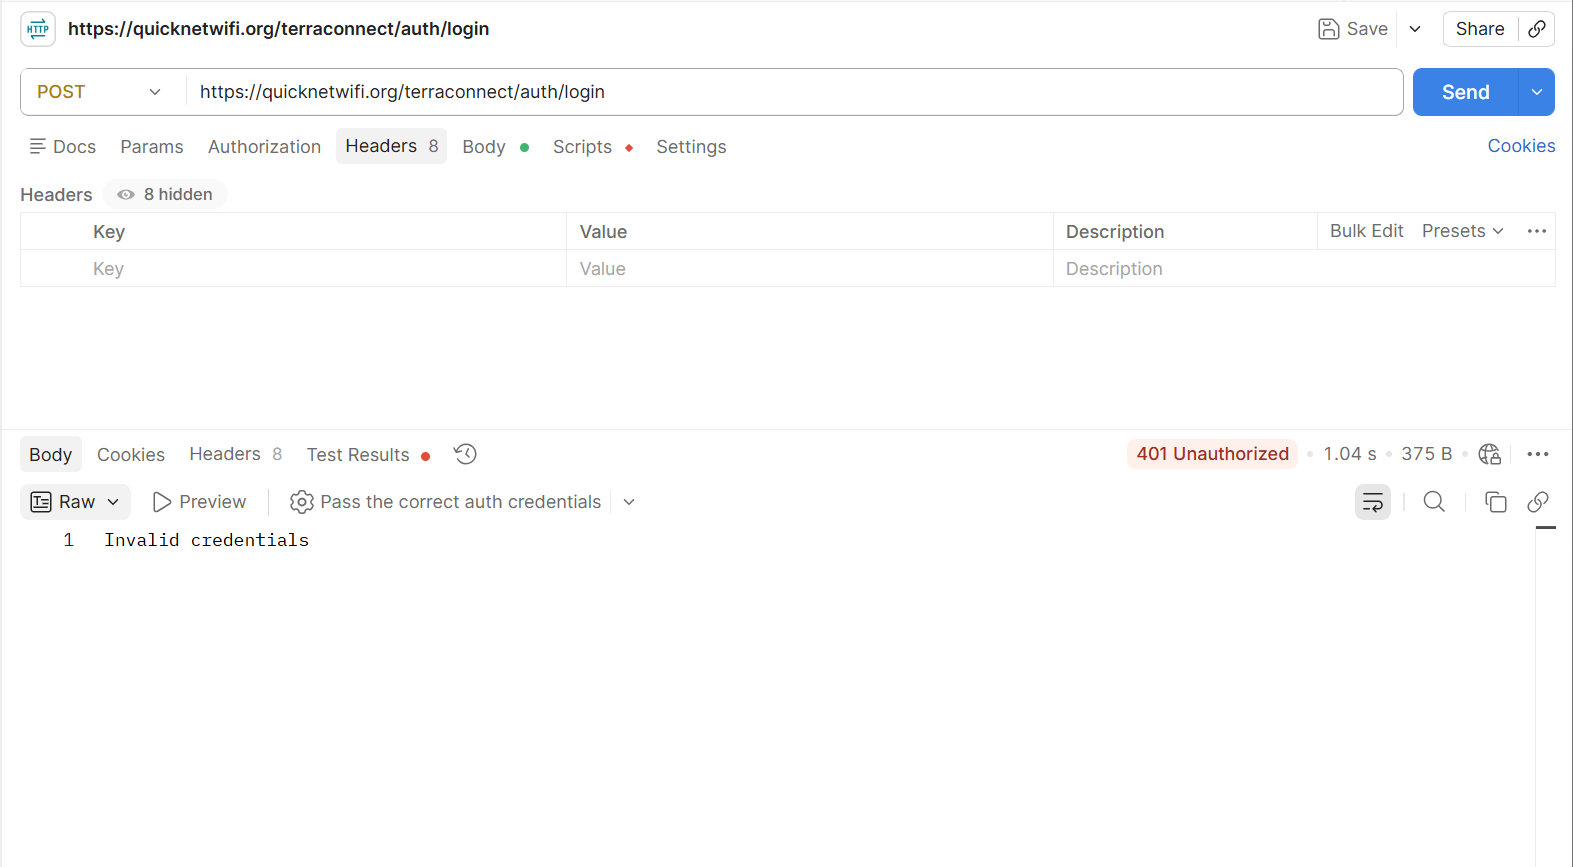
\includegraphics[width=\linewidth]{media/image5.png}
  \caption{Picture 1122}
\end{figure}



\textbf{Figure 5.1: Postman API Test: Failed Login Response (HTTP 401 Unauthorized)}


The screenshot demonstrates the backend's response to a POST request submitted with incorrect credentials to the /auth/login endpoint, returning an HTTP 401 Unauthorized status with an "Invalid credentials" error message, confirming that the authentication layer correctly rejects unauthorised access attempts.


\textbf{Postman Login Demonstration for Blocked Accounts}


\begin{figure}[htbp]
  \centering
  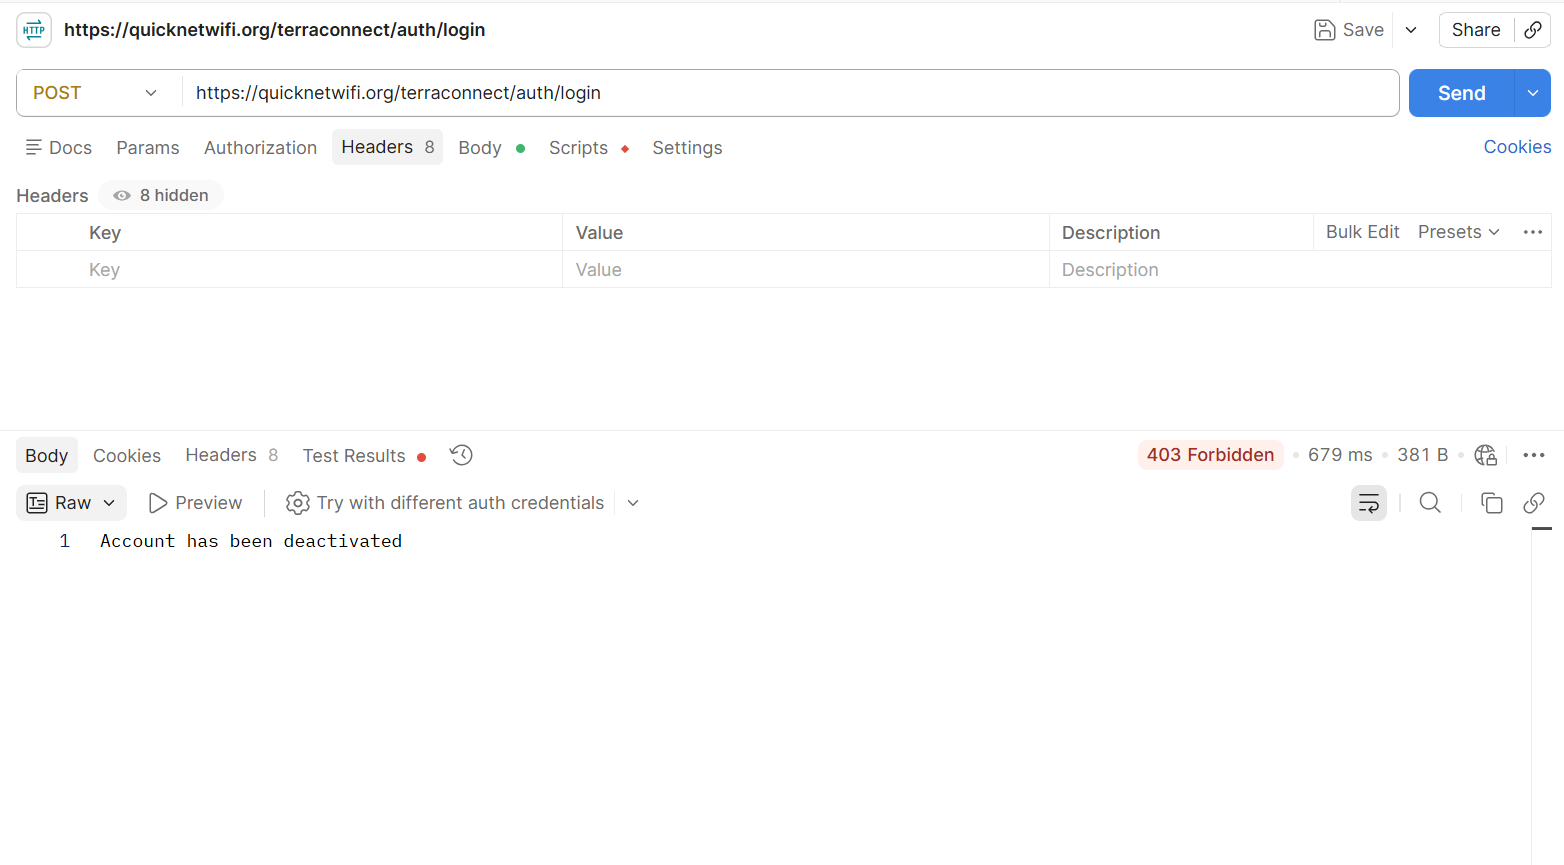
\includegraphics[width=\linewidth]{media/image6.png}
  \caption{Picture 522}
\end{figure}

\textbf{Figure 5.2: Postman API Test: Blocked Account Login Response (HTTP 403 Forbidden)}


\clearpage

The screenshot demonstrates the backend's response to a login attempt by a deactivated user account on the /auth/login endpoint, returning an HTTP 403 Forbidden status with an "Account has been deactivated" error message, confirming that the system correctly enforces access restrictions on blocked or inactive accounts.


\subsection{5.1.2 Router Onboarding Logic via the TerraConnect Uganda Mobile Application}

This section well presents the results of the implementation of the router onboarding subsystem of TerraConnect Uganda management platform.


The onboarding process enables WISP operators to register their routers into the platform directly from an android mobile application, after which the router is provisioned into an encrypted Virtual Private Network tunnel managed by the server.


\textbf{Overview of the Onboarding Architecture}


The router onboarding process was designed to satisfy two distinct deployment realities encountered during fieldwork in Uganda.


\textbf{Public IP deployment}


The router is directly reachable over the internet via a public IP address. The backend can connect to it autonomously to verify its identity and push configuration.


\textbf{CGNAT/Private IP deployment}


The router sits behind a Carrier Grade NAT or a local LAN which is the dominant scenario for small WISPs operating through the ISP internet connections. In this case the mobile application acts as the configuration bridge


\textbf{The Full Onboarding Sequence}


\begin{figure}[htbp]
  \centering
  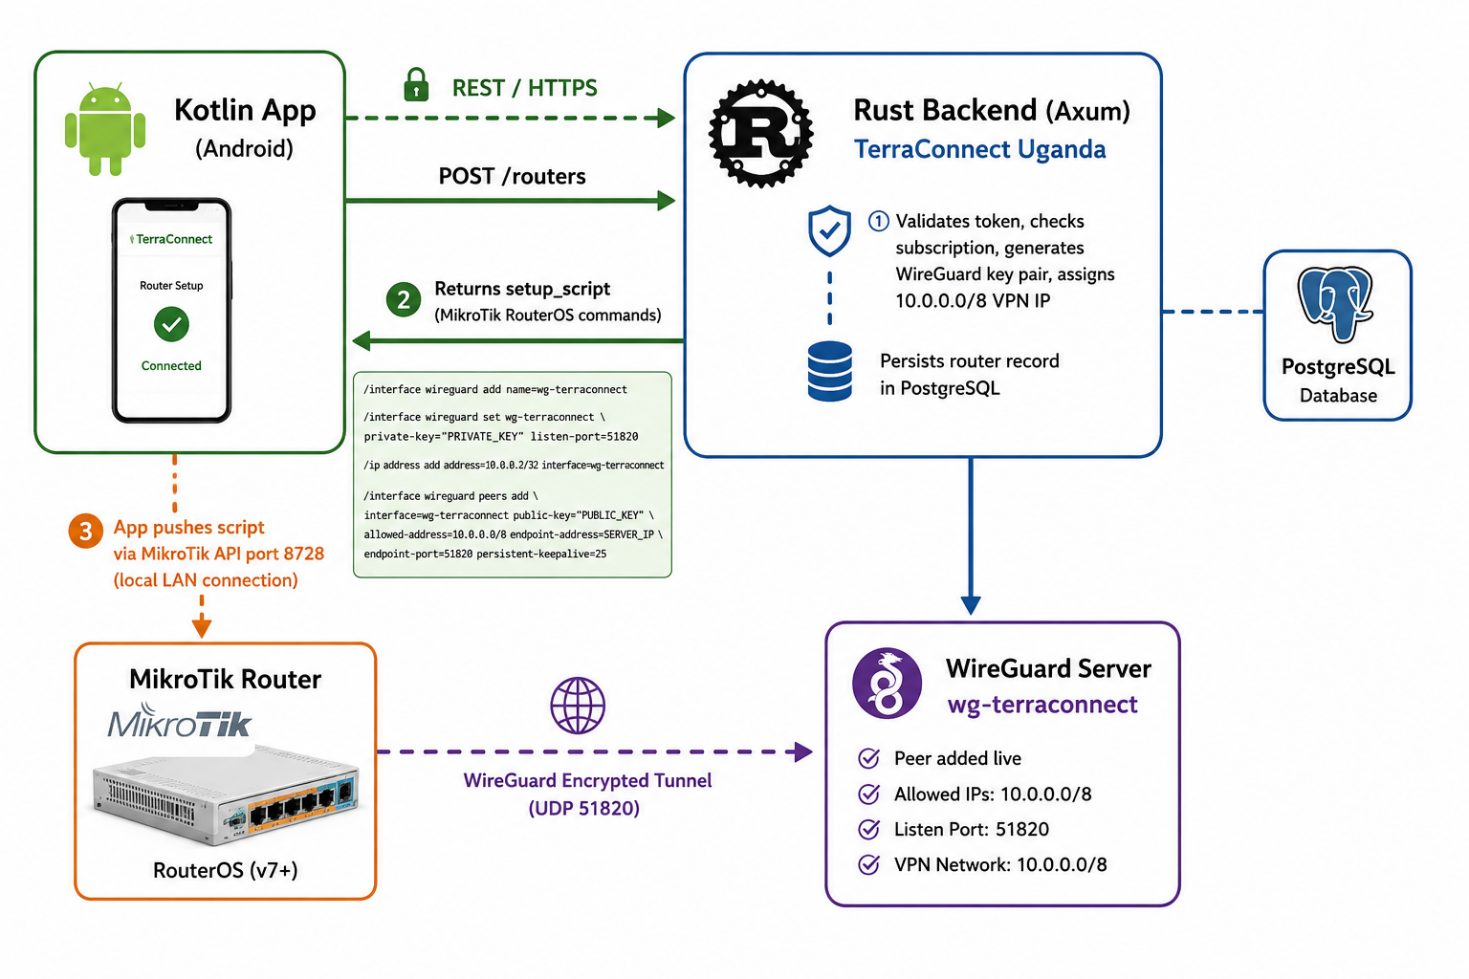
\includegraphics[width=\linewidth]{media/image7.png}
  \caption{Picture 523}
\end{figure}



\textbf{Figure 5.3: System Architecture: Router Provisioning and WireGuard Tunnel Establishment}The figure illustrates the end-to-end flow of router provisioning within the TerraConnect Uganda system. The process is initiated from the Android (Kotlin) application, which submits POST / routers request to the Rust backend via REST/HTTPS. The backend validates the user token, verifies the subscription, generates a WireGuard key pair, assigns a VPN IP address within the 10.0.0.0/8 subnet, and persists the router record in the PostgreSQL database. A RouterOS configuration script is then returned to the mobile application, which pushes it directly to the MikroTik router via the MikroTik API on port 8728 over a local LAN connection. Upon successful script execution, the MikroTik router establishes an encrypted WireGuard tunnel to the WireGuard server (wg-terraconnect) over UDP port 51820, completing the secure provisioning process.


\subsection{5.1.3 Onboarding Process }

\textbf{User Authentication}


Before any router can be registered, the operator must authenticate via the mobile application. The backend issues a JWT upon successful login. This token includes a Bearer header in all subsequent requests. Unauthenticated onboarding attempts return HTTP 401 Unauthorized confirming that the system enforces access control at the API gateway level.


\textbf{Device Identity Resolution}


The backend resolves the router identity differently depending on the network topology detected from the real\_ip field supplied when onboarding by the mobile application


When the real\_ip value is detected as a private address (RFC 1918 ranges: 10.0.0.0/8, 172.16.0.0/12, 192.168.0.0/16, or loopback 127.0.0.0/8), the backend automatically switches focus to app assisted onboarding


\begin{itemize}
  \item The application reads the routers serial number locally via the mikrotik API on port 80 over the device's LAN connection
  \item The serial number is included in the registration payload as serial\_number.
  \item The backend accepts this as proof of physical access to the device; no direct connection to the router is attempted from the server
\end{itemize}

If the serial number is absent in a NAT onboarding request, the backend returns HTTP 400 Bad Request with the message ``Serial number must be provided by the app for NAT/Private IP routers. This was a deliberate design decision to prevent registration of phantom or incorrectly identified devices.
















\textbf{Demonstration of the Onboarding Process}




\begin{figure}[htbp]
  \centering
  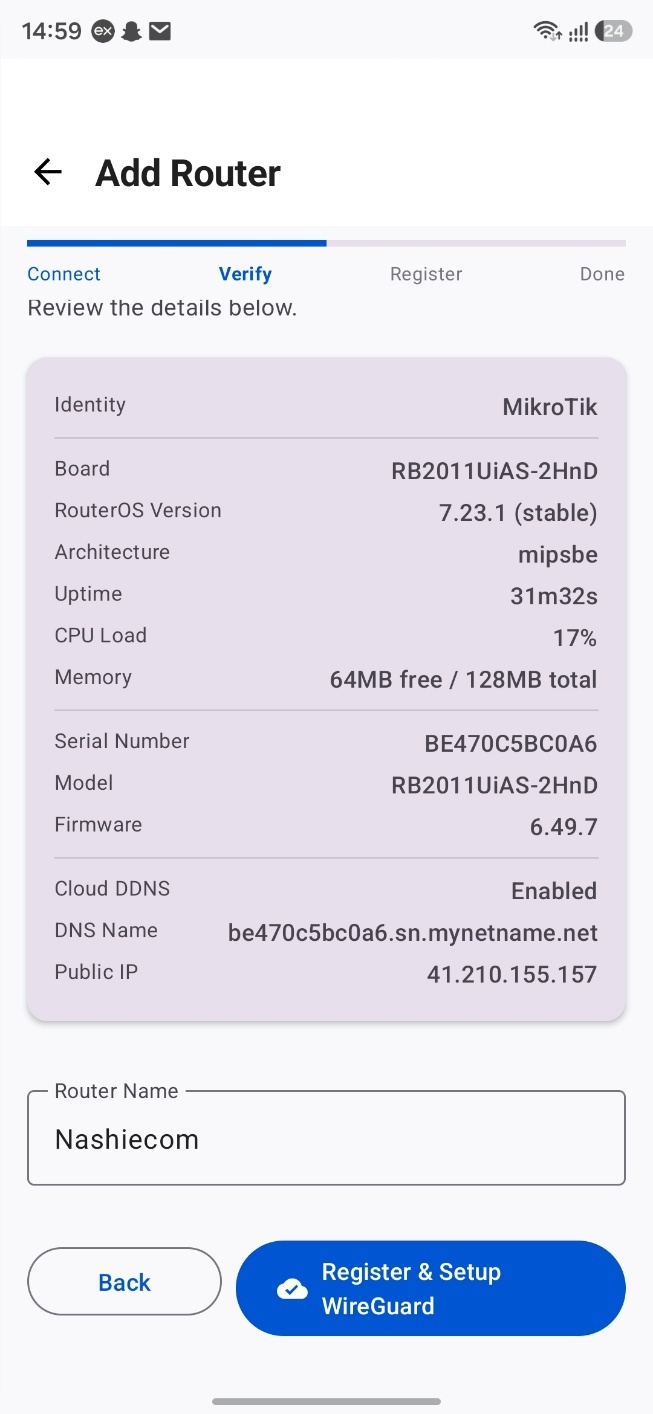
\includegraphics[width=7.43cm]{media/image8.jpeg}
  \caption{Picture 524}
\end{figure}



\textbf{Figure 5.4: Router Verification Screen: Add Router Workflow}


The screen displays the auto-detected hardware details of a MikroTik router (RB2011UiAS-2HnD) prior to registration, allowing the user to review device information including RouterOS version, CPU load, memory, and public IP before proceeding to WireGuard setup.




\begin{figure}[htbp]
  \centering
  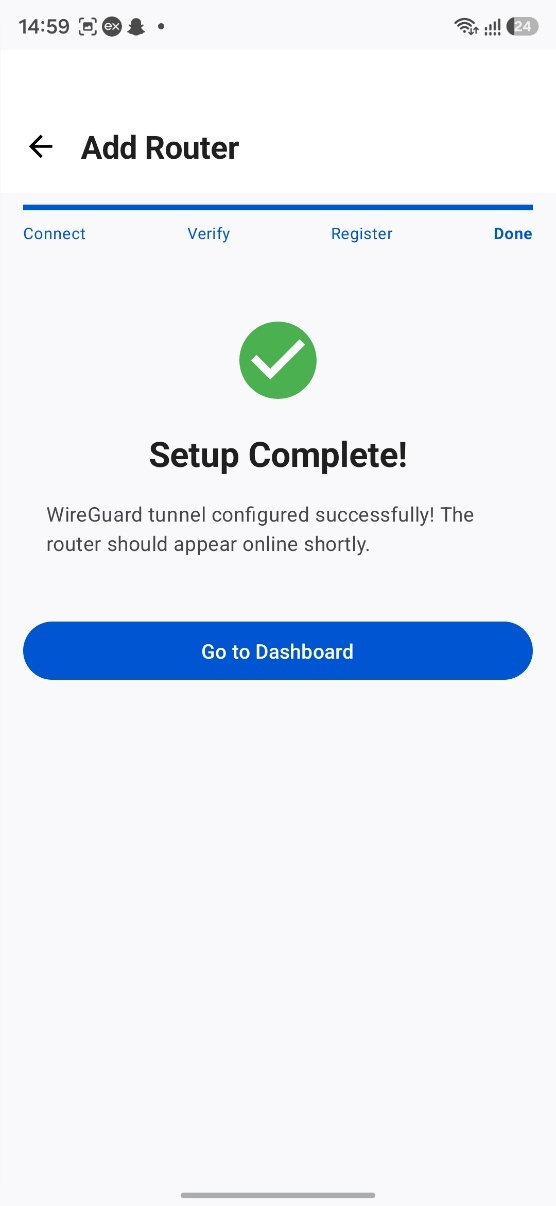
\includegraphics[width=6.39cm]{media/image9.jpeg}
  \caption{Picture 578}
\end{figure}





\textbf{Figure 5.5: Setup Completion Screen: WireGuard Tunnel Configured Successfully}


The screen above confirms the successful completion of the router registration and WireGuard tunnel configuration process, prompting the user to proceed to the dashboard where the router will appear online within the next polling interval.


\textbf{Duplicate Serial Number Check}


The system maintains a global uniqueness constraint on router serial numbers. If a serial number is already registered to any account in the database, the onboarding request returns HTTP 409 Conflict. This was verified during testing and guards against both accidental re-registration and deliberate attempts to claim another operator's router


\textbf{Wireguard Key Pair Generation and VPN IP Assignment}


Upon passing all validations, the backend generates a unique WireGuard key pair for the router using the X25519 Diffie-Hellman algorithm via the x25519-dalek crate. The keys are Base64 encoded in standard WireGuard format.


An internal VPN IP address from the 10.0.0.0/8 subnet is dynamically assigned. The assignment algorithm queries the highest currently allocated IP and increments the last octet, carrying over to the third and second octets as necessary and this supports up to 16.7 million concurrent routers. The first router onboarded receives 10.0.0.100.


A unique WireGuard listen port is also randomly generated in the range 13000 to 60000 for each router reducing NAT traversal collisions in environments where multiple routers share the same upstream public IP.


These values are persisted to the routers table in PostgreSQL atomically within a single INSERT transaction.




\textbf{WireGuard Setup Script Generation}


Upon successful database insertion, the backend generates a complete Mikrotik RouterOS script containing all commands required to bring the router into the VPN. The script is returned in all API responses as the setup\_script field.


For NAT deployed routers, the kotlin application receives this script and pushes it to the router over the local Mikrotik API connection via port 8728, completing the provisioning loop without requiring any external reachability to the router from the server. 


For public IP routers, the backend optionally performs an auto push of the configuration directly from the server after a second identity verification pass.




\textbf{Live Peer Registration on the Wireguard Server}


Immediately after the router record in inserted, the server adds the new router as a live WireGuard peer by updating the wireguard interface and executing a hot-reload(without dropping existing tunnels). The PeerManager component is idempotent and it removes any existing peer with the same public key or conflicting IP allocation before appending the new entry, preventing configuration drift over repeated onboarding attempts.


For routers on private Ips, the allowed Address routes are set to include the router's LAN subnet hence enabling the backend to reach devices on the router's downstream LAN once the tunnel is established.




\textbf{Summary of Onboarding Results}


The router onboarding subsystem of TerraConnect Uganda was successfully implemented and verified across all planned scenarios. The system correctly enforces authentication, device identity and duplicate prevention. For NAT-deployed routers, the most common case in the Ugandan context, the kotlin mobile application serves as a secure local configuration bridge returning a Mikrotik RouterOS script that the app pushes directly to the device. Upon completion, the router is registered in the central PostgreSQL database provisioned as a WireGuard VPN peer and immediately begins reporting live status metrics to the management dashboard




\textbf{Successfully Connected Router peers}


\begin{figure}[htbp]
  \centering
  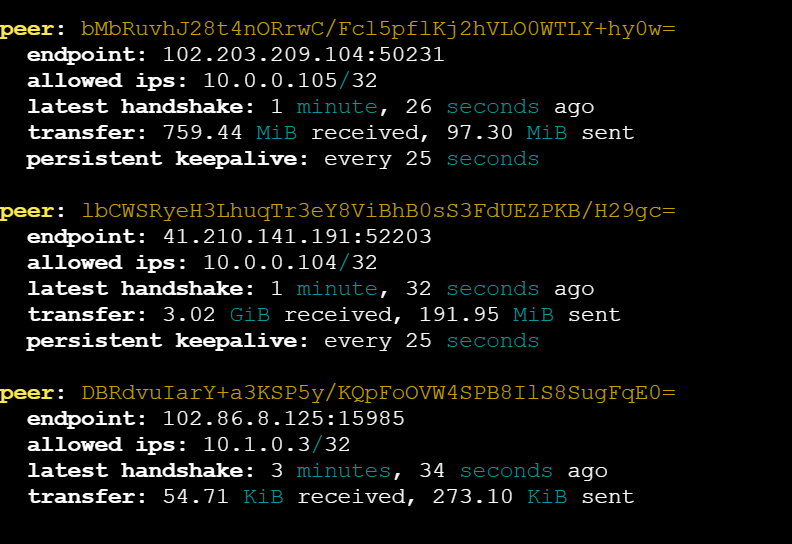
\includegraphics[width=13.97cm]{media/image10.png}
  \caption{Picture 579}
\end{figure}



\textbf{Figure 5.6: WireGuard Server Peer Status Output}The terminal output above displays the live status of three active WireGuard peers, showing each peer's public key, endpoint IP address, assigned VPN IP, time since last handshake, data transfer statistics, and persistent keepalive interval, confirming successful tunnel establishment across multiple connected routers.


\textbf{Live Ping Stats of a single router}


\begin{figure}[htbp]
  \centering
  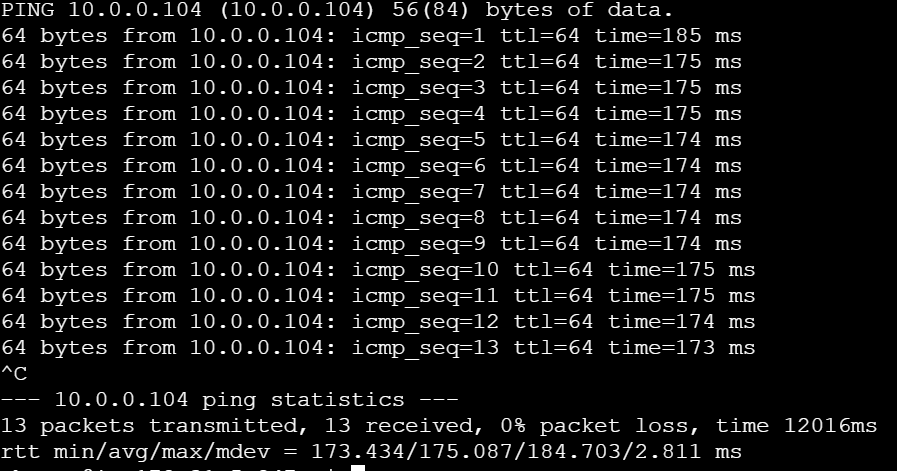
\includegraphics[width=\linewidth]{media/image11.png}
  \caption{Picture 580}
\end{figure}





\textbf{Figure 5.7: ICMP Ping Test: VPN Tunnel Latency Verification}The terminal output above shows the results of a ping test conducted to VPN peer 10.0.0.104 across the WireGuard tunnel. All 13 packets were transmitted and received successfully, recording 0\% packet loss with a consistent round-trip time averaging 175.08 ms, confirming stable and reliable tunnel connectivity under active network conditions.




\section{5.2 Integration Testing}

Integration tests exercise the full HTTP request/response cycle through the real Axum router, against a live PostgreSQL database with real JWT middleware, real password hashing and real database writes. These tests are primary mechanism for verifying that all system layers interact correctly end to end.




\section{5.3 System testing}

The system is designed for concurrent multi-tenant workloads. The PostgreSQL connection pool is configured to accept 50 maximum connections, 5 minimum connections, 10 seconds acquisition timeout and 600 seconds idle timeout. Multiple tests were ran to ensure this metric is well validated.












\section{5.4 User Acceptance Testing}

User acceptance testing was conducted with over 14 stakeholder groups corresponding to the system's roles


\textbf{User/Admin (primary role)}


Users interact with the system through the react frontend and were asked to perform the following workflow tasks


\textbf{Table 5.2: Usability Testing Results Summary}


The table below presents the outcomes of usability testing conducted on core system functionalities. Each task was performed by test users to evaluate the system's ease of use, responsiveness, and correctness of output under realistic operating conditions.


\begin{table}[htbp]
  \centering
  {\small
  \begin{tabular}{|p{6.66cm}|p{8.00cm}|}
    \hline
    Task & Result \\
    \hline
    Register, Verify Email and log in & Completed without assistance \\
    Add a Mikrotik router and view live status & Completed and router status reflected within polling interval \\
    View Traffic analytics and router logs & Completed and data populated via the NetFlow and syslog workers \\
    \hline
  \end{tabular}
  }
\end{table}



\chapter{Chapter 6: CONCLUSION AND RECOMMENDATIONS}

\section{6.1 Conclusion}

This project successfully demonstrates the development of a secure, automated, and efficient system for managing MikroTik routers that are located behind Carrier-Grade NAT (CGNAT). By leveraging Rust for the backend, the system benefits from high performance, memory safety, and concurrency, making it reliable for managing multiple routers simultaneously.


Through the integration of RouterOS API and WireGuard VPN\textbf{, }the project overcomes traditional CGNAT limitations, enabling remote access\textbf{, }configuration, and monitoring of routers without relying on public IPs or third-party vendor services. The system automates peer creation, establishes secure tunnels, and provides a monitoring mechanism to track tunnel status and connectivity in real time.


Testing and evaluation confirmed that the system is capable of:


1. Automating RouterOS configurations remotely.


2. Maintaining reliable WireGuard tunnels across NAT restrictions. 3. Handling reconnection and monitoring for uptime assurance.




All in All, the project achieves its main objectives: providing a vendor-independent, secure, and programmable solution for remote router management and bridging the gap left by existing solutions like MikroTik's Back-To-Home. The methodology, tools, and implementation provide a robust foundation for further enhancements\textbf{, }such as adding a full web-based admin interface, multi-router orchestration, or scaling for enterprise deployments.


This project demonstrates that combining Rust, RouterOS automation\textbf{, }and WireGuard VPN offers a practical and efficient solution for modern network management challenges, particularly in regions where CGNAT is common.






\section{6.2 References}

1. \textbf{Al-Ani, A. A., \& Othman, M. (2020). }A review of Carrier Grade Network Address Translation (CGNAT) and its security implications. \textit{International Journal of Computer Networks \& Communications (IJCNC), 12}(5), 45--56.


2. \textbf{Ashraf, M., \& Latif, S. (2020). }Security considerations in automated network configuration systems. \textit{Journal of Network and Computer Applications, 158}(4), 102--118. \href{https://doi.org/10.1016/j.jnca.2020.102118}{\uline{https://doi.org/10.1016/j.jnca.2020.102118}}


3. \textbf{AWS Documentation. (2023). }\textit{Deploying WireGuard on EC2 for remote access}. Amazon Web Services. Retrieved\textit{ }from \href{https://docs.aws.amazon.com/}{\uline{https://docs.aws.amazon.com}}


4. \textbf{Cloudflare. (2022). }\textit{What is Carrier-Grade NAT (CGNAT)? }Retrieved from \href{https://www.cloudflare.com/learning/network-layer/what-is-cgnat/}{\uline{https://www.cloudflare.com/learning/network-layer/what-is-cgnat/}}


5. \textbf{Davidson, J., Kim, S., \& Clarke, A. (2021). }Performance and memory safety comparison of modern systems languages: Rust, Go, and C++. \textit{Software: Practice \& Experience, 51}(7), 1523-- 1541. \href{https://doi.org/10.1002/spe.2973}{\uline{https://doi.org/10.1002/spe.2973}}


6. \textbf{DigitalOcean. (2023). }\textit{How to set up WireGuard on Ubuntu}. Retrieved from \href{https://www.digitalocean.com/community/tutorials/how-to-set-up-wireguard-on-ubuntu}{\uline{https://www.digitalocean.com/community/tutorials/how-to-set-up-wireguard-on-ubuntu}}


7. \textbf{Donenfeld, J. (2018). }WireGuard: Next generation kernel network tunnel. \textit{WireGuard Whitepaper}.


8. \textbf{Donenfeld, J. (2020). }WireGuard: Next generation secure network tunnel. Retrieved from \href{https://www.wireguard.com/papers/wireguard.pdf}{\uline{https://www.wireguard.com/papers/wireguard.pdf}}


















9. \textbf{Fielding, R. T. (2000). }\textit{Architectural styles and the design of network-based software architectures }(Doctoral dissertation). University of California, Irvine.


10.\textbf{Gong, X., Li, J., \& Xu, Y. (2018). }Lightweight protocols for resource-constrained network devices. \textit{IEEE Internet of Things Journal, 5}(6), 4309--4320. \href{https://doi.org/10.1109/JIOT.2018.2865179}{\uline{https://doi.org/10.1109/JIOT.2018.2865179}}


11.\textbf{Herzberg, G., Patel, R., \& Khanna, R. (2022). }NAT traversal challenges in modern mobile networks: A measurement study. \textit{Computer} \textit{Networks, 204}, 108--123. \href{https://doi.org/10.1016/j.comnet.2021.108123}{\uline{https://doi.org/10.1016/j.comnet.2021.108123}}


12.\textbf{Klabnik, S., \& Nichols, C. (2018). }\textit{The Rust programming language}. No Starch Press.


13.\textbf{Kumar, S., \& Singh, R. (2021). }VPN technologies: A comparative analysis of IPSec, OpenVPN, and WireGuard. \textit{Journal of Network and Computer Applications, 188}, 103081. \href{https://doi.org/10.1016/j.jnca.2021.103081}{\uline{https://doi.org/10.1016/j.jnca.2021.103081}}


14.\textbf{Kurose, J. F., \& Ross, K. W. (2021). }\textit{Computer networking: A top-down approach }(8th ed.). Pearson.


15.\textbf{Mason, L. (2020). }*Practical WireGuard deployment patterns on IPv4-only networks*. Network Engineering Blog.


16.\textbf{MikroTik. (2022). }\textit{RouterOS REST API documentation}. MikroTik Documentation Portal. Retrieved from \href{https://help.mikrotik.com/}{\uline{https://help.mikrotik.com/}}


17.\textbf{MikroTik. (2023). }\textit{Cloud Hosted Router (CHR) and Back-To-Home documentation}. Retrieved from \href{https://mikrotik.com/}{\uline{https://mikrotik.com}}


18.\textbf{MikroTik. (2024). }\textit{RouterOS API reference}. Retrieved from \href{https://help.mikrotik.com/docs/display/ROS/API}{\uline{https://help.mikrotik.com/docs/display/ROS/API}}


19.\textbf{Mozilla Foundation. (2023). }\textit{Why Rust? Performance, reliability, and productivity}. Retrieved from \href{https://foundation.rust-lang.org/}{\uline{https://foundation.rust-lang.org}}












20.\textbf{Rust Foundation. (2024). }\textit{The Rust programming language documentation}. Retrieved from \href{https://doc.rust-lang.org/}{\uline{https://doc.rust-lang.org}}


21.\textbf{Schmidt, M., \& Wuttke, A. (2019). }Automation frameworks for distributed network device configuration. \textit{International Journal of Computer Networks \& Communications, 11}(4), 1--16.


22.\textbf{Sokolov, D., \& Komarov, P. (2022). }Automation of MikroTik devices using RouterOS API. In \textit{2022 International Conference on Smart Technologies (IEEE SmartTech)}. IEEE.


23.\textbf{Wijaya, A., Prasetyo, F., \& Limantara, A. (2020). }Automation of MikroTik RouterOS using programmable interfaces. \textit{Journal of Information Systems Engineering and Business Intelligence, 6}(2), 111-- 119. \href{https://doi.org/10.20473/jisebi.6.2.111-119}{https://doi.org/10.20473/jisebi.6.2.111-119}


24.\textbf{Wright, S., \& Samuels, J. (2021). }Comparative performance evaluation of WireGuard, OpenVPN, and IPsec. \textit{Journal of Cybersecurity and Network Performance, 9}(3), 44--53.


25.\textbf{Wright, S., \& Samuels, J. (2021). }Comparative performance evaluation of WireGuard, OpenVPN, and IPsec. \textit{Journal of Cybersecurity and Network Performance, 9}(3), 44--53.


26.\textbf{(Sahu \& Misra, 2020): }Supports the claim about the usability and security challenges for non-technical users.


27.\textbf{(Google, 2023): }References the official Android developer documentation on background services and networking, validating the technical feasibility.


28.\textbf{(Huang et al., 2022): }Provides research evidence for the effectiveness of using mobile APIs and specific protocols (WebSockets/MQTT) for this bridging role.








\end{document}
